% !TEX root = ../waves.tex
%%%%%%%%%%%%%%%%%%%%%%%%%%%%%%%%%%%%%%%%%%%%%%%%%%%%%%%%%%%%%%%%%%%%%%%%%%%%%%%%%%%%%%%%%%
\section{General properties of periodic functions}
A physical quantity $f(t)$ depending on a variable $t$ is said to be \emph{oscillating} or
\emph{periodic} if it repeats itself identically after a certain duration. In mathematical
terms:
\begin{definition}
  A function $f$ of a single real variable is said to be~\emph{periodic} or specifically
  \emph{$\tau$-periodic} if there exists a positive real number $\tau$ such that
  \begin{equation}
    \forall t\in\mathbb{R},\quad f(t+\tau)=f(t)\,.
  \end{equation}
  $\tau$ is called a \emph{period} of $f$.
\end{definition}
\noindent For example, $\sin(t)$ is $2\pi$-periodic, and a constant function admits any
number has a period. Another fundamental quantity is the \emph{frequency}:
\begin{definition}
  If $\tau$ is a period of a given function $f$, its inverse
  \begin{equation}
    \omega=\frac{1}{\tau}
  \end{equation}
  is called a \emph{frequency} of $f$.
\end{definition}
\noindent In physical terms, if $t$ is a time variable, $\tau$ is also a time, and
$\omega$ is the number of oscillations per unit of time. One can notice that a periodic
function never has a unique period, \eg clearly if $\tau$ is a period, $2\tau$ is also a
period. Because of this it is useful to write the following definition
\begin{definition}
  The infimum $\tau_0$ of the set of all possible periods of a given periodic function $f$
  is called the \emph{fundamental period} of $f$. The associated frequency
  $\omega_0=\frac{1}{\tau_0}$ is called the \emph{fundamental frequency} of $f$.
\end{definition}
\noindent For example, the fundamental frequency of $\sin(t)$ is $2\pi$, and it is zero
for a constant function. Another fundamental quantity is the \emph{amplitude} of a
periodic function, measuring the size of the oscillations within a fundamental period:
\begin{definition}
  \label{def:amplitude}
  Let $f$ be a real periodic function with fundamental period $\tau_0$. We additionally
  assume that $f$ is bounded with infimum and supremum
  \begin{equation}
    m=\inf_{0\leq t\leq \tau_0}f(t)\qquad\text{and}\qquad M=\sup_{0\leq t\leq \tau_0}f(t)\,.
  \end{equation}
  The \emph{amplitude} of $f$ is then defined by
  \begin{equation}
    A=\frac{M-m}{2}\,.
  \end{equation}
\end{definition}
\noindent For example, the amplitude of $\sin(t)$ is equal to $1$, and it is zero for
constant functions. \cref{def:amplitude} assumes that $f$ is bounded, and one can question
whether this hypothesis is true in general. It is not, but continuity is a sufficient
condition:
\begin{proposition}
  If a real periodic function is continuous, then it is bounded (and therefore it has a
  well-defined amplitude).
\end{proposition}
\begin{proof}
  Let $f$ be a continuous $\tau$-periodic function. Since $f$ is continuous on the compact
  interval $[0,\tau]$, it follows from the boundedness theorem that it is also bounded on
  this interval. Finally, using the periodicity, any value $f(t)$ is equal to a value
  $f(t_0)$ with $0\leq t_0\leq \tau_0$, therefore $f$ is bounded.
\end{proof}
\noindent One can show that this condition is not necessary, \ie discontinuous periodic
functions can be bounded as well. One example of such function is the \emph{square wave},
that will be useful later:
\begin{definition}
  \label{def:sq-wave}
  The square wave function $\sq(t)$ is defined by
  \begin{equation}
    \sq(t)=
    \begin{cases}
      1, &\text{if~}\lfloor 2t\rfloor~\text{is even}\\
      -1, &\text{if~}\lfloor 2t\rfloor~\text{is odd}\\
    \end{cases}\,,
    \label{eq:wave-square}
  \end{equation}
  where $\lfloor t\rfloor$ is the floor function, \ie the largest integer smaller or equal
  to $t$.
\end{definition}
\noindent It is left as an exercise to the reader to show that $\sq(t)$ is periodic with
fundamental period $1$ and amplitude $1$, and can be rewritten as
\begin{equation}
  \sq(t)=2(2\lfloor t\rfloor-\lfloor 2t\rfloor)+1\,.
\end{equation}
Additionally, $\sq(t)$ is discontinuous at all points of the form $t=\frac{n}{2}$ where
$n\in\mathbb{Z}$. The curve of $\sq(t)$ is represented in~\cref{fig:sq-wave}.
\begin{figure}[t]
  \centering
  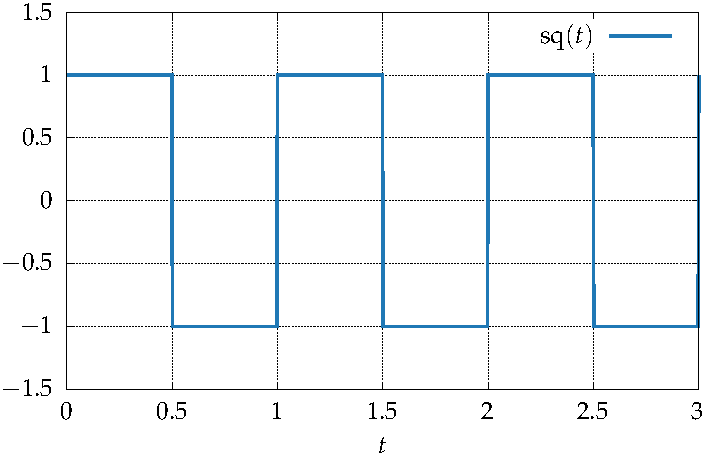
\includegraphics{gp_sq-wave.pdf}
  \caption{Curve of the square wave defined in~\cref{def:sq-wave}.}
  \label{fig:sq-wave}
\end{figure}

As anticipated in the previous chapter, fundamental building blocks for periodic functions
are the sine and cosine functions, which is the essence of Fourier analysis. It is
therefore useful to familiarise ourselves beforehand with periodic functions built using
sine and cosine, which is the topic of the next section.
%%%%%%%%%%%%%%%%%%%%%%%%%%%%%%%%%%%%%%%%%%%%%%%%%%%%%%%%%%%%%%%%%%%%%%%%%%%%%%%%%%%%%%%%%%
\section{Elementary waves}
We start by defining elementary sine waves
\begin{definition}
  \label{def:sine-wave}
  We call \emph{elementary sine wave} the function defined by
  \begin{equation}
    \sw(t;\omega,\phi)=\sin(2\pi\omega t + \phi)\,.\label{eq:sine-wave}
  \end{equation}
  where $\omega\neq 0$ and $0\leq\phi<2\pi$ are the \emph{frequency} and \emph{phase} of
  the wave, respectively. When the phase argument is omitted then it is assumed that
  $\phi=0$, \ie $\sw(t;\omega)=\sw(t;\omega,0)$.
\end{definition}
\noindent It is straightforward to show that, according to the definition in the previous
section, $\sw(t;\omega,\phi)$ is a periodic function with fundamental frequency $|\omega|$
and amplitude $1$. The phase measures the delay in the oscillation relatively to a wave
with identical frequency equal to zero at $t=0$. More generally if two waves have
identical frequencies and different phases $\phi_1$ and $\phi_2$, the time delay between
them is given by
\begin{equation}
  \delta t =\frac{\tau}{2\pi}\delta\phi\qquad\text{with}\qquad\delta\phi=\phi_1-\phi_2\,,
\end{equation}
with the fundamental period $\tau=\frac{1}{\omega}$. More explicitly,
\begin{equation}
  \sw(t;\omega,\phi_1)=\sw(t+\delta t;\omega,\phi_2)\,.
\end{equation}
In other words, the phase can always be re-written as a shift in time:
\begin{equation}
  \sw(t;\omega,\phi)=\sw(t+t_0;\omega),
  \qquad\text{with}\qquad
  t_0 = \frac{\tau\phi}{2\pi}\,.\label{eq:phase-delay}
\end{equation}
The frequency and phase are represented graphically in~\cref{fig:sine-wave}.
\begin{figure}[t]
  \centering
  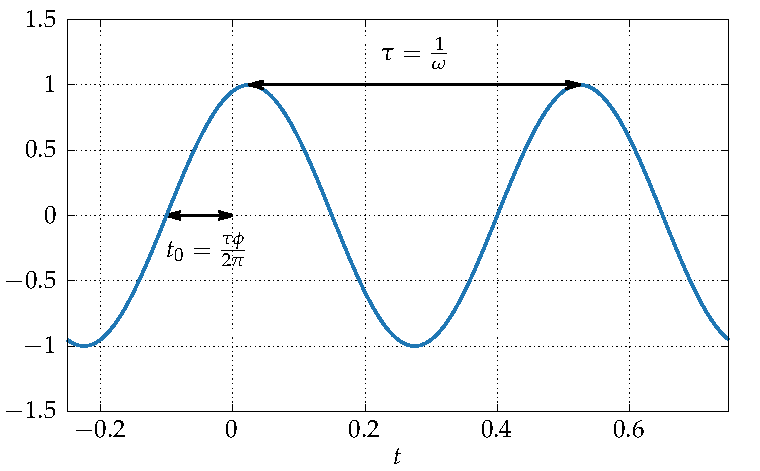
\includegraphics{gp_sine-wave.pdf}
  \caption{Example curve of the sine wave defined in~\cref{eq:sine-wave}, with frequency
    $\omega=2$ and phase $\phi=0.2\times 2\pi$. The arrows represent the period $\tau$ and
  the phase delay from~\cref{eq:phase-delay}.}
  \label{fig:sine-wave}
\end{figure}
For the special phase $\frac{\pi}{2}$, a sine wave can be written using the cosine
function:
\begin{equation}
  \sw\left(t;\omega,\frac{\pi}{2}\right)= \cos(2\pi\omega t)\,,
\end{equation}
motivating the following definition
\begin{definition}
  \label{def:cosine-wave}
  We call \emph{elementary cosine wave} the function
  \begin{equation}
    \cw(t;\omega,\phi)=\cos(2\pi\omega t + \phi)\,.\label{eq:cosine-wave}
  \end{equation}
  Similarly to the case of sine waves we define $\cw(t;\omega)=\cw(t;\omega,0)$. Sine and
  cosine waves are related by the following phase relationships
  \begin{equation}
    \sw(t;\omega,\phi)=\cw\left(t;\omega,\phi-\frac{\pi}{2}\right),
    \quad\text{and}\quad
    \cw(t;\omega,\phi)=\sw\left(t;\omega,\phi+\frac{\pi}{2}\right)\,.
  \end{equation}
\end{definition}
A crucial set of formula to manipulate waves is given by the angle addition theorem:
\begin{theorem}[Angle addition]
  \label{thm:angle-add}
  For all pairs of real numbers $a$ and $b$, the following identities hold
  \begin{align}
    \sin(a+b)&=\sin(a)\cos(b)+\cos(a)\sin(b)\,,\label{eq:sinapb}\\
    \sin(a-b)&=\sin(a)\cos(b)-\cos(a)\sin(b)\,,\label{eq:sinamb}\\
    \cos(a+b)&=\cos(a)\cos(b)-\sin(a)\sin(b)\,,\label{eq:cosapb}\\
    \cos(a-b)&=\cos(a)\cos(b)+\sin(a)\sin(b)\,.\label{eq:cosamb}
  \end{align}
\end{theorem}
\begin{proof}
  We remind that the sine and cosine function are the real and imaginary part of the
  exponential of a purely imaginary number, namely for all $\theta\in\mathbb{R}$,
  \begin{equation}
    e^{i\theta}=\cos(\theta)+i\sin(\theta)\,.
  \end{equation}
  Therefore,
  \begin{equation}
    e^{i a}e^{i b}=\cos(a)\cos(b)-\sin(a)\sin(b)+i[\cos(a)\sin(b)+\sin(a)\cos(b)]\,,
    \label{eq:eaeb}
  \end{equation}
  and by definition
  \begin{equation}
    e^{i(a+b)}=\cos(a+b)+i\sin(a+b)\,.\label{eq:eapb}
  \end{equation}
  Now, using the fact that $e^{i(a+b)}=e^{i a}e^{i b}$, and identifying the real and
  imaginary parts in~\cref{eq:eaeb,eq:eapb}, one directly
  obtains~\cref{eq:sinapb,eq:cosapb}. \cref{eq:sinamb,eq:cosamb} can then be obtained
  using the parity properties of the sine and cosine functions, namely $\sin(-x)=-\sin(x)$
  and $\cos(-x)=\cos(x)$.
\end{proof}
These identities
\begin{corollary}
  \label{cor:sumproduct}
  For all pairs of real numbers $a$ and $b$, the following identities hold
  \begin{align}
    \sin(a)\sin(b)&=\frac{1}{2}\left[\cos(a-b)-\cos(a+b)\right]\,,
    \label{eq:sinatsinb}\\
    \sin(a)\cos(b)&=\frac{1}{2}\left[\sin(a-b)+\sin(a+b)\right]\,,
    \label{eq:sinatcosb}\\
    \cos(a)\cos(b)&=\frac{1}{2}\left[\cos(a-b)+\cos(a+b)\right]\,,
    \label{eq:cosatcosb}\\
    \sin(a)+\sin(b)&=2\sin\left(\frac{a+b}{2}\right)\cos\left(\frac{a-b}{2}\right)\,,
    \label{eq:sinapsinb}\\
    \cos(a)+\cos(b)&=2\cos\left(\frac{a+b}{2}\right)\cos\left(\frac{a-b}{2}\right)\,.
    \label{eq:cosapcosb}
  \end{align}
\end{corollary}
\begin{proof}
  \cref{eq:sinatsinb,eq:cosatcosb} are obtained by considering the sum and difference
  of~\cref{eq:cosapb,eq:cosamb}, and~\cref{eq:sinatcosb} by taking the sum
  of~\cref{eq:sinapb,eq:sinamb}. Then, we define
  \begin{equation}
    c=\frac{a+b}{2}\qquad\text{and}\qquad d=\frac{a-b}{2}\,,
  \end{equation}
  which implies that $a=c+d$ and $b=c-d$. Now, using~\cref{eq:sinatcosb} leads to
  \begin{align}
    \sin(a)+\sin(b)&=\sin(c+d)+\sin(c-d)=2\sin(c)\cos(d)\notag\\
    &=2\sin\left(\frac{a+b}{2}\right)\cos\left(\frac{a-b}{2}\right)\,,
  \end{align}
  which proves~\cref{eq:sinapsinb}. \cref{eq:cosapcosb} can be derived in the same way
  using~\cref{eq:cosatcosb}.
\end{proof}
These additional formulas allow to systematically convert a product of sine/cosine
functions into a sum, and vice-versa. The angle addition theorem can be proven solely
using triangle geometry, which is significantly less trivial than the simple proof above,
based on complex numbers. Elementary waves can generally be easier to manipulate using
complex exponentials, motivating the definition below.
\begin{definition}
  \label{def:complex-wave}
  We call \emph{elementary complex wave} the function
  \begin{equation}
    \ew(t;\omega,\phi)=e^{i(2\pi\omega t + \phi)}\,.
  \end{equation}
  As previously we define $\ew(t;\omega)=\ew(t;\omega,0)$. By definition of the complex
  exponential, elementary complex waves are related to sine and cosine elementary waves by
  the relation
  \begin{equation}
    \ew(t;\omega,\phi)=\cw(t;\omega,\phi)+i\,\sw(t;\omega,\phi)\,,
  \end{equation}
  Thanks to the properties of the exponential, we have the two following trivial
  relationships
  \begin{equation}
    \ew(t;\omega,\phi)=e^{i\phi}\ew(t;\omega)\,\quad\text{and}\quad
    \ew(t;\omega,\phi)^*=\ew(-t;\omega,-\phi)=\ew(t;-\omega,-\phi)\,,\label{eq:cw-conj}
  \end{equation}
  Using these formulas, the relationship to sine and cosine waves can be rewritten as
  \begin{align}
    \cw(t;\omega,\phi)&=\frac{1}{2}[\ew(t;\omega,\phi)+\ew(t;-\omega,-\phi)]\,,
    \label{eq:cwtoew}\\
    \sw(t;\omega,\phi)&=-\frac{i}{2}[\ew(t;\omega,\phi)-\ew(t;-\omega,-\phi)]\,.
    \label{eq:swtoew}
  \end{align}
\end{definition}
A considerable simplification with complex waves comes from the fact that the phase just
leads to a multiplicative factor, equivalent to giving a \emph{complex amplitude} to the
wave. Similarly, phased sine and cosine waves can be expressed as a sum of zero-phase ones
using the angle addition theorem:
\begin{align}
  \sw(t;\omega,\phi)&=\cos(\phi)\sw(t;\omega)+\sin(\phi)\cw(t;\omega)\,,\\
  \cw(t;\omega,\phi)&=\cos(\phi)\cw(t;\omega)-\sin(\phi)\sw(t;\omega)\,.
\end{align}
%%%%%%%%%%%%%%%%%%%%%%%%%%%%%%%%%%%%%%%%%%%%%%%%%%%%%%%%%%%%%%%%%%%%%%%%%%%%%%%%%%%%%%%%%%
\section{Combination of elementary waves}
We will now discuss how to create more general waves by adding elementary waves. One first
legitimate question is whether the sum of two periodic functions is till periodic. It is
not always true, and can be characterised by the following result:
\begin{theorem}
  \label{thm:period-sum}
  Let $f_1(t)$ and $f_2(t)$ be two periodic functions of fundamental periods $\tau_1\neq
  0$ and $\tau_2\neq 0$, respectively. Then the sum $f_1+f_2$ as well as the product
  $f_1f_2$ are periodic if and only if the period ratio  $\smash{\frac{\tau_1}{\tau_2}}$
  is a rational number.
  % If this condition is true, this ratio can be written
  % $\smash{\frac{\tau_1}{\tau_2}}=\smash{\frac{p}{q}}$ where $p$ and $q$ are two coprime
  % integers (\ie their GCD is $1$), and the fundamental frequency $\tau$ of $f(t)$ is
  % given by \begin{equation} \tau=q\tau_1=p\tau_2\,. \end{equation}
\end{theorem}
\begin{proof}
  % TODO
\end{proof}
\begin{example}
  \label{ex:period-sum}
  $\sin\left(\frac{2\pi}{3}t\right)+\sin(\pi t)$ is periodic with fundamental period $6$.
\end{example}
\begin{example}
  \label{ex:nperiod-sum}
  $\sin(t)+\sin(\pi t)$ is not periodic.
\end{example}
\noindent Both examples above are illustrated in~\cref{fig:sine-sum}. Mathematically
speaking,~\cref{thm:period-sum} means that generally periodic functions sums are not
periodic. However, we remind the reader that any real number is arbitrarily close to a
rational number, so non-periodic sums like in~\cref{ex:nperiod-sum} can always be
approximated arbitrarily well by a periodic function. This is relevant for physics and
engineering applications where quantities are often known up to some limited precision.
\begin{figure}[t]
  \centering
  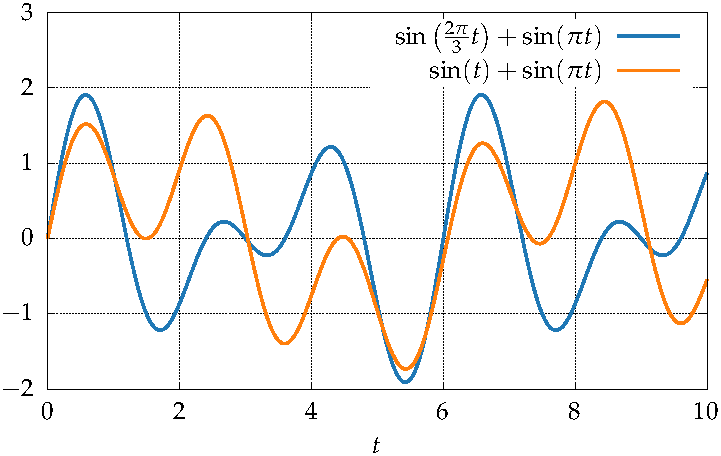
\includegraphics{gp_sine-sum.pdf}
  \caption{Curves of the sine wave sums in~\cref{ex:period-sum,ex:nperiod-sum}}
  \label{fig:sine-sum}
\end{figure}

Regarding elementary waves, one can demonstrate easily using the angle addition theorem
that products can always be reduced to sums:
\begin{proposition}
  The following identities hold for multiplying elementary waves:
  \begin{align}
    \cw(\omega_1)\cw(\omega_2)&=\frac{1}{2}[\cw(\omega_1-\omega_2)+\cw(\omega_1+\omega_2)]
    \label{eq:cprod}\\
    \sw(\omega_1)\sw(\omega_2)&=\frac{1}{2}[\cw(\omega_1-\omega_2)-\cw(\omega_1+\omega_2)]
    \label{eq:sprod}\\
    \sw(\omega_1)\cw(\omega_2)&=\frac{1}{2}[\sw(\omega_1-\omega_2)+\sw(\omega_1+\omega_2)]
    \label{eq:scprod}\\
    \ew(\omega_1)\ew(\omega_2)&=\ew(\omega_1+\omega_2)\label{eq:eprod}
  \end{align}
\end{proposition}
\begin{proof}
  These identities are a trivial re-interpretation of~\cref{cor:sumproduct}.
\end{proof}

An important concept when adding waves is the notion of \emph{interference}. Waves
oscillate between negative and positive values (or around the unit circle for complex
waves), and can add up or cancel when summed. This can be formalised in the following way
\begin{definition}
  Let $f$ and $g$ be two complex-valued periodic functions, not necessarily with the same
  period. We consider the sum $h=f+g$, which modulus squared is given by
  \begin{equation}
    |h|^2=|f|^2+|g|^2+2\Re(f^*g)\,.
  \end{equation}
  The last term $2\Re(f^*g)$ in the equation is called the \emph{interference term}. At a
  given point $t\in\mathbb{R}$:
  \begin{enumerate}
    \item if $\Re[f^*(t)g(t)]>0$, $f$ and $g$ are said to \emph{interfere constructively}
      at $t$;
    \item if $\Re[f^*(t)g(t)]<0$, $f$ and $g$ are said to \emph{interfere destructively}
      at $t$.
  \end{enumerate}
  If $f$ and $g$ are real-valued functions, the interference term is simply given by
  $2fg$.
\end{definition}
We now discuss below key examples of interference between elementary waves.
\begin{example}
  We consider the sum of two sine waves with equal frequencies, but different phases:
  \begin{equation}
    f(t)=\sw(t;\omega)+\sw(t;\omega,\phi)\,.
  \end{equation}
  Using~\cref{eq:sinapsinb}, $f(t)$ can be re-written as
  \begin{equation}
    f(t)=2\cos\left(\frac{\phi}{2}\right)\sw\left(t;\omega,\frac{\phi}{2}\right)\,.
  \end{equation}
  So $f$ is still an elementary sine wave with frequency $\omega$, phase $\frac{\phi}{2}$,
  and amplitude $2\cos(\frac{\phi}{2})$. The interesting element here is the change of
  amplitude: at $\phi=0$, the amplitude of $f$ is $2$, and the two waves interfere in a
  maximally constructive way, they are said to be \emph{in phase}. At $\phi=\pi$, $f$ is
  identically zero and the two waves interfere in a maximally destructive way, they are
  said to be \emph{out of phase}. Using the definition above, and~\cref{eq:sinatsinb}, the
  related interference term is given by
  \begin{equation}
    2\sw(t;\omega,\phi)\sw(t;\omega)=\cos(\phi)-\cw(t;2\omega,\phi)\,.
  \end{equation}
  Because the cosine function oscillate between $-1$ and $1$, the expression above takes
  values between $-2$ and $2$. If $\phi=0$, the two waves interfere constructively for all
  $t$, which is the maximally constructive case above. Similarly, the waves interfere
  destructively for all $t$ with $\phi=\pi$. This example is illustrated
  in~\cref{fig:interference}
\end{example}
\begin{figure}[ph!]
  \centering
  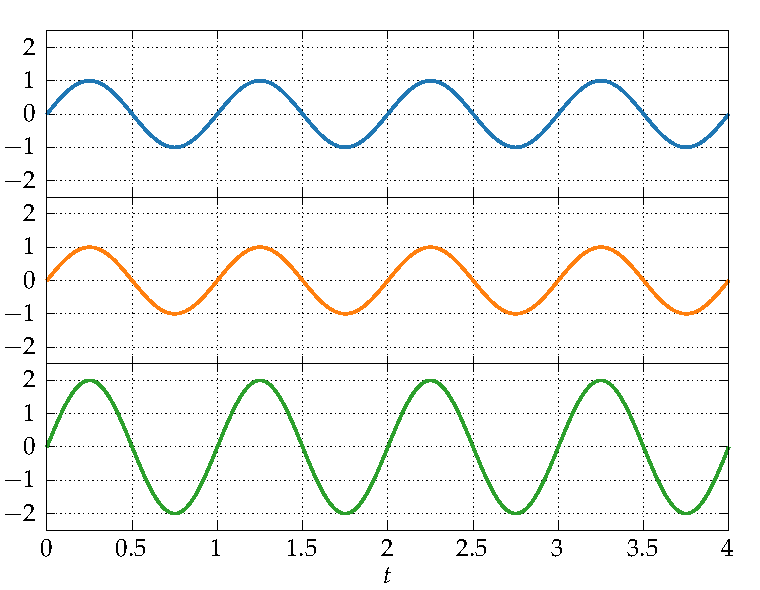
\includegraphics{gp_sine-interference.pdf}
  \\\hspace{0.2cm}(a)\\~\\
  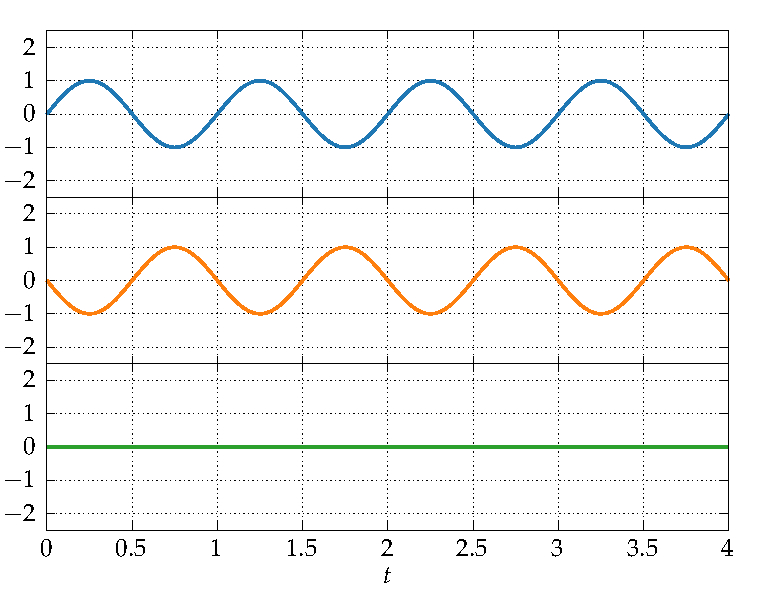
\includegraphics{gp_sine-interference-des.pdf}
  \\\hspace{0.2cm}(b)\\
  \caption{For each figure above, the lowermost curve represent the sum of the two curves
    above. Pane (a) represents a case of maximally constructive interference between two
    in-phase sine waves with frequency $1$. Pane (b) represents a case of maximally
  destructive interference between two out-of-phase sine waves with frequency $1$.}
  \label{fig:interference}
\end{figure}
\begin{example}
  Another important example of interference is the \emph{beating effect}, which occurs
  when summing two elementary waves with slightly different frequencies:
  \begin{equation}
    f(t)=\sw(t;\omega)+\sw(t;\omega+\delta\omega)\,,
  \end{equation}
  where $\delta\omega$ is assumed to be small compared to $\omega$. In this case, the
  interference term can be written
  \begin{equation}
    2\sw(t;\omega)\sw(t;\omega+\delta\omega)=\cw(t;\delta\omega)-\cw(t;2\omega+\delta\omega)
    \simeq \cw(t;\delta\omega)-\cw(t;2\omega)\,,
  \end{equation}
  where in the last term we used the assumption on the smallness of $\delta\omega$. The
  first cosine in this expression oscillates much slower than the second one, and is equal
  to $1$ for $t=\smash{\frac{n}{\delta\omega}}$, and $-1$ for
  $t=\smash{\frac{n}{\delta\omega}+\frac{1}{2\delta\omega}}$. Following the same argument
  as in the previous example, this means that $f(t)$ oscillates in time between maximally
  constructive and destructive interference, at the frequency $\delta\omega$. This is
  generally called a \emph{beating effect}, particularly in an acoustic context, where the
  intensity of the sound associated to $f(t)$ very distinctly goes to zero periodically
  $\delta\omega$ times per second.

  Another way to present this phenomenon is to write the identity
  \begin{equation}
    f(t)=2\cw\left(t;\frac{\delta\omega}{2}\right)
    \sw\left(t;\omega+\frac{\delta\omega}{2}\right)
    \simeq 2\cw\left(t;\frac{\delta\omega}{2}\right)\sw(t;\omega)\,.
  \end{equation}
  In that form, $f(t)$ appears as a sine wave with frequency $\omega$ modulated by a
  cosine with half this frequency. Since the cosine function goes to zero twice per
  period, we find again that $f(t)$ goes to zero with frequency $\delta\omega$. The
  beating effect is illustrated in~\cref{fig:beating}.
\end{example}
\begin{figure}
  \centering
  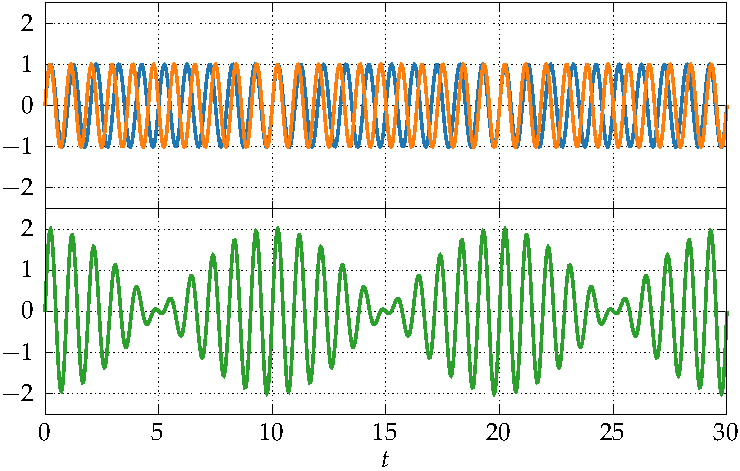
\includegraphics{gp_sine-beating.pdf}
  \caption{The upper plot represents two sine waves with slightly different frequencies
    $\omega=1$ and $\omega+\delta\omega=1.1$. The lower plot represents the sum of these
    two waves, with a visible beating effect with frequency $\delta\omega=0.1$. The beats
  can be correlated with the two sine waves going in and out of phase.}
  \label{fig:beating}
\end{figure}
%%%%%%%%%%%%%%%%%%%%%%%%%%%%%%%%%%%%%%%%%%%%%%%%%%%%%%%%%%%%%%%%%%%%%%%%%%%%%%%%%%%%%%%%%%
\section{Trigonometric polynomials}
We can make the following definition for an arbitrary linear combination of elementary
waves:
\begin{definition}
  We call \emph{trigonometric polynomial} of degree $N$ and frequency $\omega$ any
  function of the form
  \begin{equation}
    P(t)=\frac{a_0}{2}+\sum_{n=1}^N[a_n\cw(t;n\omega)+b_n\sw(t;n\omega)]\,,
    \label{eq:trigp-sc}
  \end{equation}
  where $a_n$ and $b_n$ are real coefficients such that $a_N\neq 0$ or $b_N \neq 0$. The
  formula above is called the \emph{sine-cosine form} of $P(t)$ with \emph{sine-cosine
  coefficients} or \emph{modes} $a_n$ and $b_n$. The $\frac{1}{2}$ normalisation of $a_0$
  is arbitrary, and will be convenient later. It is also convenient to define $b_0=0$, to
  avoid constantly treating the $a_n$ coefficients separately for having an $n=0$
  coefficient.
\end{definition}
It is clear that such function is periodic, and a consequence of~\cref{thm:period-sum} is
then
\begin{proposition}
  Let $P$ be a trigonometric polynomial of degree $N\geq 1$ and frequency $\omega$ with
  sine-cosine coefficients $a_n$ and $b_n$. $P$ is a periodic function with period
  $\tau=\frac{1}{\omega}$, and additionally if $a_1\neq0$ or $b_1\neq0$, then $\omega$ is
  the fundamental frequency of $P(t)$.
\end{proposition}
\begin{proof}
  Each term in~\cref{eq:trigp-sc} is trivially $T$-periodic, so $P$ is also
  $\tau$-periodic. Now, the $n$-th mode of $P$ has a fundamental period of
  $\tau_n=\frac{\tau}{n}$. Assuming that $a_1\neq0$ or $b_1\neq0$, then the period ratio
  of this first mode to an arbitrary non-vanishing higher mode $n$ is given by
  \begin{equation}
    \frac{\tau_1}{\tau_n}=n\,.
  \end{equation}
  Using~\cref{thm:period-sum}, this means that this combination of modes has fundamental
  period $\tau$. The remaining modes can then be added one after another, and repeated use
  of~\cref{thm:period-sum} demonstrate the proposition.
\end{proof}
As we previously did for the elementary waves, trigonometric polynomials can be put in a
convenient complex form
\begin{definition}
  \label{def:trigp-complex}
  Let $P$ be a trigonometric polynomial of degree $N$ and frequency $\omega$ with
  sine-cosine coefficients $a_n$ and $b_n$. $P$ can be written in the \emph{complex form}
  \begin{equation}
    P(t)=\sum_{n=-N}^{N}c_n\ew(t;n\omega)\,,\label{eq:trigp-complex}
  \end{equation}
  with the \emph{complex coefficients}
  \begin{equation}
    c_n =
    \begin{cases}
      \frac{1}{2}(a_n-ib_n)&\text{if~}n< 0\\
      \frac{1}{2}(a_n+ib_n)&\text{if~}n\geq 0
    \end{cases}
    \,,\label{eq:ab-to-c}
  \end{equation}
  which have the property $c_n^*=c_{-n}$. The relation above can be inverted to
  \begin{equation}
    a_n=c_n+c_{-n}\qquad\text{and}\qquad
    b_n=i(c_n-c_{-n})\,.
  \end{equation}
\end{definition}
The formulas in the definition above can be obtained using~\cref{eq:cwtoew,eq:swtoew} with
the definition~\cref{eq:trigp-sc}, which is left as an exercise to the reader. A key
property of trigonometric polynomials, that will be crucial later, is the unicity of their
coefficients, formulated in the theorem below
\begin{theorem}
  \label{thm:trigp-unicity}
  Let $P$ and $Q$ be two trigonometric polynomials with the same frequency $\omega$,
  degrees $N$ and $N'$, and sine-cosine coefficients $a_n$,$b_n$ and $a'_n$,$b'_n$,
  respectively. $P$ and $Q$ are identically equal,~\ie $P(t)=Q(t)$ for all
  $t\in\mathbb{R}$, if and only if their degrees and coefficients are equal, \ie $N=N'$
  and for all $n$
  \begin{equation}
    a_n=a'_n\quad\text{and}\quad b_n=b'_n\,.
  \end{equation}
\end{theorem}
Although we could attempt to prove that directly, this theorem is a consequence of
fundamental orthogonality properties of elementary waves. Because these properties are
crucial in Fourier analysis, we  study them in detail in the next section, where the
theorem above will be proven.

%%%%%%%%%%%%%%%%%%%%%%%%%%%%%%%%%%%%%%%%%%%%%%%%%%%%%%%%%%%%%%%%%%%%%%%%%%%%%%%%%%%%%%%%%%
\section{Orthogonality of elementary waves}
The reader might be more familiar with the notion of orthogonality in vector spaces, which
we summarise below as an introduction to the notion of orthogonality of periodic
functions. In vector calculus, given an $n$-dimensional real vector $\vec{v}$ and a unit
vector $\vec{u}$, the \emph{orthogonal projection} $\vec{v}_{\vec{u}}$ of $\vec{v}$ on the
axis defined by $\vec{u}$ is given by
\begin{equation}
  \label{eq:orth-proj}
  \vec{v}_{\vec{u}}=\cos(\theta)|\vec{v}|\,\vec{u}\,,
\end{equation}
where $\theta$ is the angle between $\vec{u}$ and $\vec{v}$, and $|\vec{v}|$ is the norm
of $\vec{v}$. The projection coefficient $\cos(\theta)|\vec{v}|$ is known to be given by
the
\emph{dot product}
\begin{equation}
  \vec{v}\cdot \vec{u}=\sum_{j=1}^n \vec{v}_j \vec{u}_j=\cos(\theta)|\vec{v}|\,.
  \label{eq:vec-dot}
\end{equation}
Additionally, the dot product $\vec{v}\cdot \vec{u}$ vanishes when $\vec{v}$ and $\vec{u}$
are \emph{orthogonal} (\ie they form an angle of $\pi$ radians). This makes the dot
product an essential tool of vector calculus to compute the coordinate of vectors in an
orthonormal basis. Explicitly, let $\vec{e}_j$ be an orthonormal basis of $\mathbb{R}^n$,
and let $v^{\vec{e}}_j$ be the coefficients of $\vec{v}$ in that basis, \ie
\begin{equation}
  \vec{v}=\sum_{j=1}^{n}v^{\vec{e}}_j\,\vec{e}_j\,,
\end{equation}
then the $v^{\vec{e}}_j$ can be computed using the dot product using
\begin{equation}
  v^{\vec{e}}_j=\vec{v}\cdot \vec{e}_j\,.\label{eq:basis-proj}
\end{equation}
The concept of orthogonality and orthogonal projection can be generalised to more complex
mathematical objects like functions. As we discuss below, elementary waves can be
interpreted as an orthogonal basis for trigonometric polynomial, which is the reason
why~\cref{thm:trigp-unicity} holds, and a key structure at the heart of Fourier analysis.
Although the general description of orthogonality between functions is out of the scope of
this course and will not be treated here, this introduction to Fourier analysis can be
seen as a good introduction to this type of concept.
\begin{figure}[t]
  \caption{Visual representation of the orthogonal projection of a vector on a unit vector
  given in~\cref{eq:orth-proj}}
  \label{fig:orth-proj}
\end{figure}

We start by defining the dot product between two periodic functions
\begin{definition}
  \label{def:func-dot}
  Let $f$ and $g$ two real $\tau$-periodic functions. We assume that $f$ and $g$ are
  integrable on the interval $[0,\tau]$. The \emph{dot product} $\braket{f,g}$ between $f$
  and $g$ is the real number defined by
  \begin{equation}
    \braket{f,g}=\int_{0}^{\tau}\diff t\, f(t)g(t)\,.\label{eq:func-dot}
  \end{equation}
  Additionally, the \emph{$2$-norm} $\|f\|$ of the function $f$ is defined by
  \begin{equation}
    \|f\|^2=\braket{f,f}=\int_{0}^{\tau}\diff t\, f(t)^2\,.
  \end{equation}
\end{definition}
The definition~\cref{eq:func-dot} can be interpreted as a continuous version
of~\cref{eq:vec-dot}, where the values $f(t)$ and $g(t)$ are the ``continuous
coordinates'' of the functions $f$ and $g$, and the integral is a ``continuous sum'' over
these coordinates. The functional dot product has the same linearity and commutativity
properties than the vector dot product:
\begin{proposition}
  Let $f$, $g$, and $h$ be three real $\tau$-periodic functions. The following identities
  hold for any pair of real number $\alpha$ and $\beta$
  \begin{align}
    \braket{\alpha f+\beta g,h}&=\alpha\braket{f,h}+\beta\braket{g,h}\,,\\
    \braket{f,\alpha g+\beta h}&=\alpha\braket{f,g}+\beta\braket{f,h}\,,\\
    \braket{f,g}&=\braket{g,f}\,.
  \end{align}
\end{proposition}
\begin{proof}
  This is a trivial consequence of the definition~\cref{eq:func-dot} and the linearity of
  the integral.
\end{proof}
The definition of orthogonality follows naturally:
\begin{definition}
  \label{def:dot-rfunc}
  Let $f$ and $g$ be two $\tau$-periodic functions. $f$ and $g$ are said to be
  \emph{orthogonal} if their dot product vanishes, \ie
  \begin{equation}
    \braket{f,g}=0\,.
  \end{equation}
\end{definition}
We now give the main result of this section, \ie the orthogonality of elementary waves
\begin{theorem}
  \label{thm:sc-orth}
  Let $\omega>0$ be an arbitrary frequency corresponding to the period $\tau$. For any
  pair of integers $n$ and $m$, the following identities hold
  \begin{align}
    \braket{\sw(n\omega),\sw(m\omega)}&=\frac{\tau}{2}\delta_{nm}\,,\label{eq:sw-orth}\\
    \braket{\cw(n\omega),\cw(m\omega)}&=\frac{\tau}{2}\delta_{nm}\,,\label{eq:cw-orth}\\
    \braket{\cw(n\omega),\sw(m\omega)}&=0\,.\label{eq:scw-orth}
  \end{align}
  Where $\delta_{nm}$ is the \emph{Kronecker symbol}
  \begin{equation}
    \delta_{nm}=
    \begin{cases}
      1&~\mathrm{if}~~n=m\\
      0&~\mathrm{else}
    \end{cases}\,.
  \end{equation}
  In other words, for any pair of integers $n$ and $m$, sine waves of the form
  $\sw(n\omega)$ and $\sw(m\omega)$ have norm squared $\frac{\tau}{2}$ and are orthogonal
  if and only if $n\neq m$, the same applies to cosine waves, and a sine and a cosine wave
  of the form $\sw(n\omega)$ and $\cw(m\omega)$ are always orthogonal.
\end{theorem}
\begin{proof}
  Let us demonstrate~\cref{eq:sw-orth,eq:cw-orth,eq:scw-orth} using the
  definition~\cref{eq:func-dot}. We start with~\cref{eq:sw-orth}
  \begin{equation}
    \braket{\sw(n\omega),\sw(m\omega)}=\int_{0}^{\tau}\diff t\,
    \sin(2\pi n\omega t)\sin(2\pi m\omega t)\,.
  \end{equation}
  Using~\cref{eq:sprod}, one has
  \begin{equation}
    \sw(n\omega)\sw(m\omega)=\frac{1}{2}\{\cw[(n-m)\omega]-\cw[(n+m)\omega]\}\,.
    \label{eq:sw-prod}
  \end{equation}
  If $n=m$, this product simplifies to
  \begin{equation}
    \sw(n\omega)\sw(m\omega)=\frac{1}{2}[1-\cw(2n\omega)]\,,
  \end{equation}
  which integrates to
  \begin{equation}
    \frac{1}{2}\int_{0}^{\tau}\diff t\,[1-\cos(4\pi n\omega t)]=\frac{\tau}{2}-
    \left[\frac{1}{8\pi n\omega}\sin(4\pi n\omega t)\right]_0^\tau
    =\frac{\tau}{2}\,.
  \end{equation}
  If $n\neq m$, \cref{eq:sw-prod} integrates to
  \begin{align}
    &\frac{1}{2}\int_{0}^{\tau}\diff t\,\{\cos[2\pi(n-m)\omega t]-\cos[2\pi(n+m)\omega t]\}
    \notag\\
    &\qquad\qquad=\left[\frac{1}{2\pi(n-m)\omega}\sin[2\pi(n-m)\omega t]
    -\frac{1}{2\pi(n+m)\omega}\sin[2\pi(n+m)\omega t]\right]_0^\tau\notag\\
    &\qquad\qquad=0
  \end{align}
  Both equations above demonstrate~\cref{eq:sw-orth}. We now turn to~\cref{eq:cw-orth}, we
  start by using the product identity~\cref{eq:cprod}
  \begin{equation}
    \cw(n\omega)\cw(m\omega)=\frac{1}{2}\{\cw[(n-m)\omega]+\cw[(n+m)\omega]\}\,,
  \end{equation}
  which is identical to~\cref{eq:sw-prod} up to a sign. Retracing the steps above, the
  result for sine waves was independent of this sign, which implies that~\cref{eq:cw-orth}
  holds. Finally, using~\cref{eq:scprod}, we can write
  \begin{equation}
    \sw(n\omega)\cw(m\omega)=\frac{1}{2}\{\sw[(n-m)\omega]+\sw[(n+m)\omega]\}\,,
  \end{equation}
  which, if $n=m$, integrates to
  \begin{equation}
    \frac{1}{2}\int_{0}^{\tau}\diff t\,\sin(4\pi n\omega t)=
    \left[-\frac{1}{8\pi n\omega}\cos(4\pi n\omega t)\right]_0^T=0\,.
  \end{equation}
  In the case $n\neq m$, one obtains
  \begin{align}
    &\frac{1}{2}\int_{0}^{\tau}\diff t\,\{\sin[2\pi(n-m)\omega t]+\sin[2\pi(n+m)\omega t]\}
    \notag\\
    &\qquad\qquad=-\left[\frac{1}{2\pi(n-m)\omega}\cos[2\pi(n-m)\omega t]
    +\frac{1}{2\pi(n+m)\omega}\cos[2\pi(n+m)\omega t]\right]_0^\tau\notag\\
    &\qquad\qquad=0\,,
  \end{align}
  which demonstrates~\cref{eq:scw-orth}.
\end{proof}
One can also wonder about orthogonality properties of complex elementary waves. One issue
here is that the dot product from~\cref{def:dot-rfunc} was specifically defined for real
functions. It can be generalised to complex functions as follows
\begin{definition}
  Let $f$ and $g$ two complex $\tau$-periodic functions. We assume that $f$ and $g$ are
  integrable on the interval $[0,\tau]$. The \emph{dot product} $\braket{f,g}$ between $f$
  and $g$ is the complex number defined by
  \begin{equation}
    \braket{f,g}=\int_{0}^{\tau}\diff t\, f(t)g(t)^*\,.\label{eq:cfunc-dot}
  \end{equation}
  Additionally, the \emph{norm} $\|f\|$ of the function $f$ is the real number defined by
  \begin{equation}
    \|f\|^2=\braket{f,f}=\int_{0}^{\tau}\diff t\, |f(t)|^2\,.
  \end{equation}
\end{definition}
The generalisation is done by using a complex conjugation for the second argument of the
product, allowing the norm to remain a real positive number. Since any real number is its
own complex conjugate, this definition is clearly identical to~\cref{def:dot-rfunc} when
restricted to real functions. This generalisation has the consequence of slightly breaking
the symmetry of the dot product:
\begin{proposition}
  Let $f$, $g$, and $h$ be three complex $\tau$-periodic functions. The following
  identities hold for any pair of complex numbers $\alpha$ and $\beta$
  \begin{align}
    \braket{\alpha f+\beta g,h}&=\alpha\braket{f,h}+\beta\braket{g,h}\,,\\
    \braket{f,\alpha g+\beta h}&=\alpha^*\braket{f,g}+\beta^*\braket{f,h}\,,\\
    \braket{f,g}&=\braket{g,f}^*\,.
  \end{align}
\end{proposition}
\begin{proof}
  This is a trivial consequence of the definition~\cref{eq:cfunc-dot} and the linearity of
  the integral and complex conjugation.
\end{proof}
With this generalised dot product, we can formulate the orthogonality of complex
elementary waves
\begin{theorem}
  Let $\omega>0$ be an arbitrary frequency corresponding to the period $\tau$. For any
  pair of integers $n$ and $m$, the following identity holds
  \begin{equation}
    \braket{\ew(n\omega),\ew(m\omega)}=\tau\delta_{nm}\,,
  \end{equation}
  \ie for any pair of integers $n$ and $m$, complex elementary waves of the form
  $\ew(n\omega)$ and $\ew(m\omega)$ have norm squared $\tau$ and are orthogonal if and
  only if $n\neq m$.
\end{theorem}
\begin{proof}
  Using~\cref{eq:eprod,eq:cw-conj}, one has
  \begin{align}
    \braket{\ew(n\omega),\ew(m\omega)}&=\int_{0}^{\tau}\diff t\,\ew(t;n\omega)\ew(t;m\omega)^*
    =\int_{0}^{\tau}\diff t\,\ew(t;n\omega)\ew(t;-m\omega)\\
    &=\int_{0}^{\tau}\diff t\,e^{2\pi i (n-m)\omega t}\,.
  \end{align}
  If $n=m$, clearly
  \begin{equation}
    \braket{\ew(n\omega),\ew(m\omega)}=\tau\,,
  \end{equation}
  and if $n\neq m$
  \begin{equation}
    \braket{\ew(n\omega),\ew(m\omega)}=
    \left[\frac{1}{2\pi i (n-m)}e^{2\pi i (n-m)\omega t}\right]_0^\tau=0\,,
  \end{equation}
  which proves the theorem.
\end{proof}
One can notice, once again, that algebra is considerably simpler when using complex
elementary waves. We are now ready to prove~\cref{thm:trigp-unicity}:
\begin{proof}[Proof of~\cref{thm:trigp-unicity}]
  Let $P(t)$ and $P'(t)$ be two trigonometric polynomial of the general form
  \begin{align}
    P(t)&=a_0+\sum_{n=1}^N[a_n\,\cw(t;n\omega)+b_n\,\sw(t;n\omega)]\,,\\
    P'(t)&=a'_0+\sum_{n=1}^{N'}[a'_n\,\cw(t;n\omega)+b'_n\,\sw(t;n\omega)]\,.
  \end{align}
  We additionally assume that $P(t)$ and $P'(t)$ are identically equal, \ie
  \begin{equation}
    P(t)=P'(t)\,,
  \end{equation}
  for all real number $t$. This implies that for any integer $m$ one has
  \begin{equation}
    \braket{P,\cw(m\omega)}=\braket{P',\cw(m\omega)}\,.
  \end{equation}
  Using the orthogonality relations from~\cref{thm:sc-orth}, these dot products can be
  simplified to
  \begin{equation}
    \braket{P,\cw(m\omega)}=
    \begin{cases}
      \frac{\tau}{2}a_m&~\text{if}~m\leq N\\
      0&~\text{else}
    \end{cases},
    \quad\text{and}\quad
    \braket{P',\cw(m\omega)}=
    \begin{cases}
      \frac{\tau}{2}a'_m&~\text{if}~m\leq N'\\
      0&~\text{else}
    \end{cases}\,.
  \end{equation}
  Similarly,
  \begin{equation}
    \braket{P,\sw(m\omega)}=\braket{P',\sw(m\omega)}\,,
  \end{equation}
  and
  \begin{equation}
    \braket{P,\sw(m\omega)}=
    \begin{cases}
      \frac{\tau}{2}b_m&~\text{if}~m\leq N\\
      0&~\text{else}
    \end{cases},
    \quad\text{and}\quad
    \braket{P',\sw(m\omega)}=
    \begin{cases}
      \frac{\tau}{2}b'_m&~\text{if}~m\leq N'\\
      0&~\text{else}
    \end{cases}\,.
  \end{equation}
  Combining the equalities above implies directly that $a_n=a'_n$ and $b_n=b'_n$ for all
  $n$.
\end{proof}
We can notice that~\cref{thm:trigp-unicity} is somewhat trivial when one knows the
orthogonality relationships between sine and cosine waves. This also generalises a
well-known property from vector calculus: a set of orthogonal vectors defines a unique
coordinate system, and these coordinates can be obtained using orthogonal projection on
the basis vectors as in~\cref{eq:basis-proj}. Finally, \cref{thm:trigp-unicity}
generalises naturally to the complex form of trigonometric polynomials:
\begin{corollary}
  \label{corr:trigp-unicity-cplx}
  Let $P$ and $Q$ be two trigonometric polynomials with the same frequency $\omega$,
  degrees $N$ and $N'$, and complex coefficients $c_n$ and $c'_n$, respectively. $P$ and
  $Q$ are identically equal,~\ie $P(t)=Q(t)$ for all $t$, if and only if their degrees and
  coefficients are equal, \ie $N=N'$ and for all $n$
  \begin{equation}
    c_n=c'_n\,.
  \end{equation}
\end{corollary}
\begin{proof}
  Using~\cref{thm:trigp-unicity}, we know that the sine-cosine coefficients of the
  polynomials are unique. We also saw in~\cref{eq:ab-to-c} that complex coefficients are
  uniquely defined from the sine-cosine ones, which proves the coronary. Another way to
  prove this result is, similarly to the proof of~\cref{thm:trigp-unicity}, to project $P$
  in the form~\cref{eq:trigp-complex} on complex waves:
  \begin{equation}
    \braket{P,\ew(m\omega)}=
    \begin{cases}
      \tau c_m&~\text{if}~m\leq N\\
      0&~\text{else}
    \end{cases}\,,
  \end{equation}
  which, as previously, provides a unique determination of the $c_m$ coefficients given
  $P$.
\end{proof}
This concludes this section on the orthogonality of elementary waves. We will now discuss
how to generalise elementary waves and trigonometric polynomials to multiple real
variables.
%%%%%%%%%%%%%%%%%%%%%%%%%%%%%%%%%%%%%%%%%%%%%%%%%%%%%%%%%%%%%%%%%%%%%%%%%%%%%%%%%%%%%%%%%%
\section{Elementary waves in multiple dimensions}
In all this chapter, we discussed elementary waves and their combinations as functions of
a single real variable. However, oscillatory physical systems will often require multiple
variables to be described. We already encountered that in~\cref{chap:wave-eq} when
studying the wave equation. We found that the wave equation
solution~\cref{eq:string-fourier} for the plucked string was a periodic function both in
the time and space dimensions. Before starting to discuss how this result can help us to
define trigonometric polynomials in multiple dimensions, we need to formulate a definition
for multidimensional periodic functions. This can be done simply by considering functions
that are periodic in each of their variables:
\begin{definition}
  A function $f$ on $\mathbb{R}^d$ is said to be \emph{periodic} or specifically
  \emph{$\vec{\tau}$-periodic} if there exists a vector $\vec{\tau}$ with positive
  components such that $f(\vec{x})=f(x_1,\dots,x_d)$ is $\tau_j$-periodic in the variable
  $x_j$, for all directions $j$. The vector $\vec{\tau}$ is called a \emph{period} of $f$,
  and the vector $\vec{\omega}$ defined by
  \begin{equation}
    \omega_j=\frac{1}{\tau_j}\,,
  \end{equation}
  is called a \emph{frequency} of $f$.
\end{definition}
\begin{example}
  The function $f$ defined by $f(x,y)=\sin(x+2y)$ is $(2\pi,\pi)$-periodic.
\end{example}

\begin{figure}[t]
  \centering
  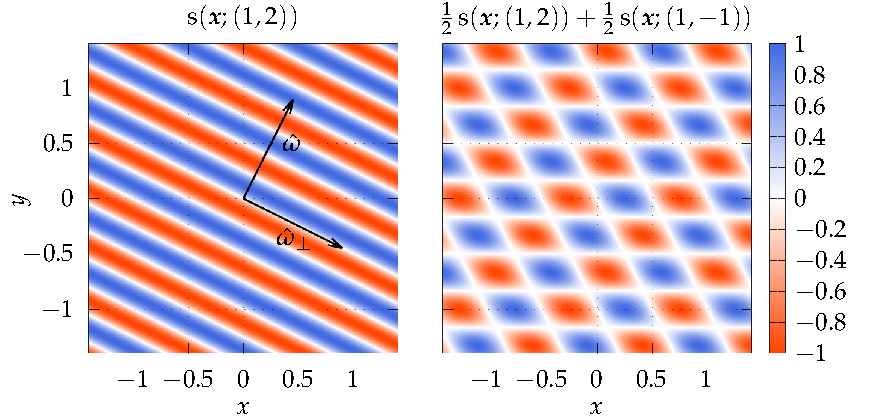
\includegraphics{gp_wave-plane.pdf}
  \caption{The left pane represents the plane wave $\sw(\vec{x};\vec{\omega})$, with
    $\vec{x}=(x,y)$ and $\vec{\omega}=(1,2)$. The arrows represent the unit vectors
    $\hat{\bm{\omega}}=(1,2)/\sqrt{5}$, and $\hat{\bm{\omega}}_{\perp}=(2,-1)/\sqrt{5}$ in
    the perpendicular direction. The right pane shows the interference pattern emerging
  when adding two plane sine waves with wave vectors $(1,2)$ and $(1,-1)$.}
  \label{fig:plane-wave}
\end{figure}
\begin{figure}[t]
  \centering
  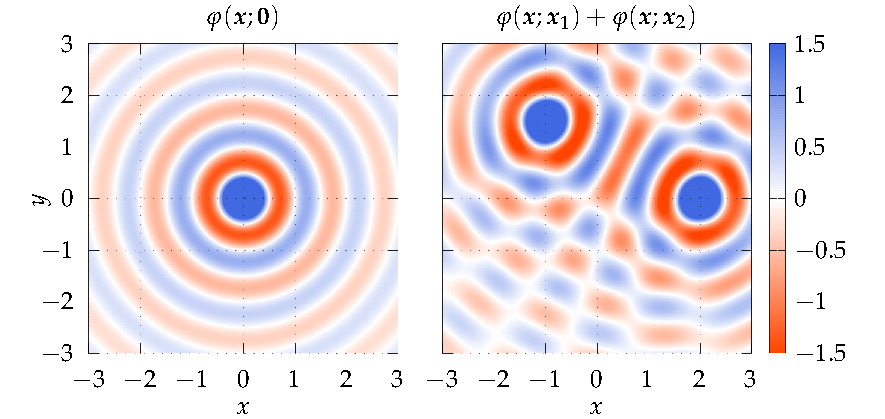
\includegraphics{gp_wave-sphere.pdf}
  \caption{The left pane represents the spherical wave $\varphi(\vec{x};\vec{0})$, with
    $\vec{x}=(x,y)$, defined in~\cref{eq:sphere-wave}. The right pane shows an example of
    interference patten between two spherical waves with source positions
    $\vec{x}_1=(-1,1.5)$ and $\vec{x}_2=(0,2)$. Although the maximum magnitude of $\varphi$
    is $2\pi=6.28$, the colour scale was limited to the interval $[-1.5,1.5]$ for
  visibility.}
  \label{fig:sphere-wave}
\end{figure}
We could inspire ourselves from the solution~\cref{eq:string-fourier} of the plucked
string problem to define trigonometric polynomials in $d$ dimensions to be linear
combinations of products of $d$ elementary sine or cosine waves. Although this would be a
fine definition, it would need a tedious discussion of the combinatorics of all the
possible independent cross-terms between sine and cosine waves. This is, once more, a
situation where using complex exponentials brings considerable simplifications, since the
product of complex waves is still a complex wave. Explicitly, assuming a vector of $d$
real variables $\vec{x}=(x_1,\dots,x_d)$, and a vector of $d$ frequencies
$\vec{\omega}=(\omega_1,\dots,\omega_d)$, we can write
\begin{align}
  e^{2\pi i\omega_1x_1}\cdots e^{2\pi i\omega_dx_d}
  &=e^{2\pi i(\omega_1x_1+\cdots+\omega_dx_d)}=e^{2\pi i\vec{\omega}\cdotp\vec{x}}\notag\\
  &=\cos(2\pi\vec{\omega}\cdot\vec{x})+i\sin(2\pi\vec{\omega}\cdot\vec{x})\,.
\end{align}
This motivates the following definitions for multidimensional elementary waves
\begin{definition}
  \label{def:multidim-waves}
  We call \emph{elementary sine wave}, \emph{elementary cosine wave}, and \emph{elementary
  complex wave} on $\mathbb{R}^d$ the functions defined by
  \begin{align}
    \sw(\vec{x};\vec{\omega},\phi)&=\sin(2\pi\vec{\omega}\cdot\vec{x}+\phi)\,,\\
    \cw(\vec{x};\vec{\omega},\phi)&=\cos(2\pi\vec{\omega}\cdot\vec{x}+\phi)\,,\\
    \ew(\vec{x};\vec{\omega},\phi)&=e^{2\pi i\vec{\omega}\cdotp\vec{x}+\phi}\,,
  \end{align}
  respectively, where the \emph{wave vector} $\vec{\omega}\in\mathbb{R}^d$ has only
  non-zero components, and the \emph{phase} $\phi$ is a real number such that $0\leq \phi
  <2\pi$.
\end{definition}
Because multidimensional elementary waves are essentially defined as one-dimensional waves
applied on a dot product, most identities from the previous section can be easily
generalised. The previous statement can be investigated further in the following way: for
a given wave vector $\vec{\omega}$, any vector $\vec{x}$ can be uniquely written as
\begin{equation}
  \vec{x}=\vec{x}_{\parallel}+\vec{x}_{\perp}\,,
\end{equation}
where $\vec{x}_{\parallel}$ is the orthogonal projection of $\vec{x}$ on $\vec{\omega}$,
and $\vec{x}_{\perp}$ is the perpendicular remainder. Explicitly
\begin{equation}
  \vec{x}_{\parallel}=(\vec{x}\cdot\hat{\vec{\omega}})\,\hat{\vec{\omega}}
  \qquad\text{and}\qquad
  \vec{x}_{\perp}=\vec{x}-\vec{x}_{\parallel}\,,
\end{equation}
where $\hat{\vec{\omega}}$ is the unit vector in the direction of $\vec{\omega}$, \ie
\begin{equation}
  \hat{\vec{\omega}}=\frac{\vec{\omega}}{|\vec{\omega}|}\,.
\end{equation}
One can check explicitly that $\vec{x}_{\perp}$ is indeed orthogonal to $\vec{\omega}$:
\begin{equation}
  \vec{x}_{\perp}\cdot\vec{\omega}
  =\vec{x}\cdot\vec{\omega}-\vec{x}_{\parallel}\cdot\vec{\omega}
  =|\vec{\omega}|(\vec{x}\cdot\hat{\vec{\omega}})
  -(\vec{x}\cdot\hat{\vec{\omega}})(\hat{\vec{\omega}}\cdot\vec{\omega})=0\,,
\end{equation}
and therefore, using sine waves as an example
\begin{equation}
  \sw(\vec{x};\vec{\omega},\phi)=\sin(2\pi\vec{\omega}\cdot\vec{x}_{\parallel}+\phi)\,.
\end{equation}
So the oscillations of a sine wave with frequency vector $\vec{\omega}$ only occur in the
direction parallel to $\vec{\omega}$, and the wave is constant in the perpendicular
direction. Assuming $\vec{x}$ is aligned with $\vec{\omega}$, \ie it can be written
$\vec{x}=z\hat{\vec{\omega}}$ with $z\in\mathbb{R}$, then
\begin{equation}
  \sw(\vec{x};\vec{\omega},\phi)=\sin(2\pi|\vec{\omega}|z+\phi)=\sw(z;|\vec{\omega}|,\phi)\,.
\end{equation}
In summary, $\sw(\vec{x};\vec{\omega},\phi)$ is a one-dimensional sine-wave of frequency
$|\vec{\omega}|$ on the axis defined by $\hat{\vec{\omega}}$, and is constant in all
perpendicular directions. In three dimensions, the perpendicular space to the wave vector
is the plane with equation $\vec{\omega}\cdot\vec{x}=0$, and for that reason the waves
defined above are generally called \emph{plane waves}. An example of two-dimensional plane
wave is given in~\cref{fig:plane-wave}.

Coming back to the wave equation, the standing wave solution~\cref{eq:stand-wave-example}
is a plane wave in space-time when written in its travelling wave
form~\cref{eq:stand-wave-travel}. Explicitly, the solution
\begin{equation}
  u(t,x)=\frac{A}{2}\left\{\sin\left[\frac{\pi}{L}n(x+ct)\right]
  +\sin\left[\frac{\pi}{L}n(x-ct)\right]\right\}\,,
\end{equation}
can be written
\begin{equation}
  u(t,x)=\frac{A}{2}[\sw(\vec{x};\vec{\omega}_n)+\sw(\vec{x};\bar{\vec{\omega}}_n)]\,,
\end{equation}
where $\vec{x}$ is the space-time vector $(ct,x)$, and the wave vectors $\vec{\omega}_n$
and $\bar{\vec{\omega}}_n$ are given by
\begin{equation}
  \vec{\omega}_n=\frac{n}{\lambda}(1,1)\qquad\text{and}\qquad
  \bar{\vec{\omega}}_n=\frac{n}{\lambda}(-1,1)\,,
\end{equation}
where $\lambda=2L$ is the wavelength. This type of reformulation using space-time
positions is fundamental in the context of special relativity, where space and time
dimensions cannot be considered independent through change of coordinates, but it is
perhaps unusual in describing non-relativistic mechanics systems.

Another class of multidimensional wave, crucial in physics, are \emph{spherical waves}.
Spherical wave are oscillatory functions which are only functions of the distance between
to points. One example that will be important later in this course is given by
\begin{equation}
  \label{eq:sphere-wave}
  \varphi(\vec{x};\vec{x}_0)=\frac{\sin(2\pi|\vec{x}-\vec{x}_0|)}{|\vec{x}-\vec{x}_0|}\,,
\end{equation}
where $\vec{x}_0$ is called the \emph{source position} of the wave. In three dimensions,
using the spherical coordinates $(r,\phi,\theta)$ centred on $\vec{x}_0$, $\varphi$
becomes
\begin{equation}
  \varphi(r,\phi,\theta)=\frac{\sin(2\pi r)}{r}\,,
\end{equation}
\ie it is a one-dimensional sine wave of frequency $1$ in any radial direction from
$\vec{x_0}$, attenuated with $\frac{1}{r}$, and is constant on any sphere with centre
$\vec{x_0}$. Such example of spherical wave is illustrated in~\cref{fig:sphere-wave}.
Finally, both in~\cref{fig:plane-wave,fig:sphere-wave} are represented examples of
interference between sums of plane waves and spherical waves, respectively. Those will be
studied further in the exercises of this chapter.

Similarly to one-dimensional elementary waves, multidimensional elementary waves are
orthogonal for distinct wave vectors. In order to show that, we need to first define an
appropriate dot product:
\begin{definition}
  Let $f$ and $g$ be two $\vec{\tau}$-periodic functions on $\mathbb{R}^d$. The \emph{dot
  product} between $f$ and $g$ is defined by
  \begin{equation}
    \braket{f,g}=\int_0^{\tau_1}\diff x_1\cdots\int_0^{\tau_d}\diff x_d\,
    f(\vec{x})g(\vec{x})^*\,.
  \end{equation}
\end{definition}
Then, the following theorem holds
\begin{theorem}
  \label{thm:nd-orth}
  Let $\vec{\omega}$ and arbitrary $d$-dimensional wave vector. For all integer vector
  $\vec{n}$, we define the \emph{component-wise product}\footnote{Sometimes referred to as
  \emph{Hadamard product}.}
  \begin{equation}
    \vec{\omega}\odot\vec{n}=(\omega_1n_1,\dots,\omega_dn_d)\,.
  \end{equation}
  The following \emph{orthogonality relation} holds for all integer vectors $\vec{n}$ and
  $\vec{m}$
  \begin{align}
    \braket{\ew(\vec{\omega}\odot\vec{n}),\ew(\vec{\omega}\odot\vec{m})}=\prod_{j=1}^{d}\delta_{n_jm_j}\tau_j\,,
  \end{align}
  with $\tau_j=\frac{1}{\omega_j}$. Additionally, if $\vec{n}$ and $\vec{m}$ only have
  components, one has
  \begin{align}
    \braket{\sw(\vec{\omega}\odot\vec{n}),\sw(\vec{\omega}\odot\vec{m})}
    &=\frac{1}{2}\prod_{j=1}^{d}\delta_{n_jm_j}\tau_j\,,\\
    \braket{\cw(\vec{\omega}\odot\vec{n}),\cw(\vec{\omega}\odot\vec{m})}
    &=\frac{1}{2}\prod_{j=1}^{d}\delta_{n_jm_j}\tau_j\,,\\
    \braket{\cw(\vec{\omega}\odot\vec{n}),\sw(\vec{\omega}\odot\vec{m})}&=0\,.
  \end{align}
\end{theorem}
This theorem will be proven in the exercises of this chapter. It is worth noting that if
the frequency is equal to $\omega>0$ in all directions, then the relationships above
simplify to
\begin{align}
  \braket{\ew(\omega\vec{n}),\ew(\omega\vec{m})}&=\tau^d\delta_{\vec{n}\vec{m}}\,,\\
  \braket{\sw(\omega\vec{n}),\sw(\omega\vec{m})}&=\frac{\tau^d}{2}\delta_{\vec{n}\vec{m}}\,,\\
  \braket{\cw(\omega\vec{n}),\cw(\omega\vec{m})}&=\frac{\tau^d}{2}\delta_{\vec{n}\vec{m}}\,,\\
  \braket{\cw(\omega\vec{n}),\sw(\omega\vec{m})}&=0\,,
\end{align}
where, as usual, $\tau=\frac{1}{\omega}$, and we generalised the \emph{Kronecker symbol}
to vectors as follows
\begin{equation}
  \delta_{\vec{n}\vec{m}}=\prod_{j=1}^{d}\delta_{n_jm_j}=
  \begin{cases}
    1&~\mathrm{if}~~\vec{n}=\vec{m}\\
    0&~\mathrm{else}
  \end{cases}\,.
\end{equation}
We can now define trigonometric polynomial in multiple dimensions:
\begin{definition}
  We call \emph{trigonometric polynomial} and wave vector $\vec{\omega}$ any function on
  $\mathbb{R}^d$ of the form
  \begin{equation}
    P(\vec{x})=\sum_{\vec{n}\in C}c_{\vec{n}}\ew(\vec{x};\vec{\omega}\odot\vec{n})
    =\sum_{\vec{n}\in C}c_{\vec{n}}\,e^{2\pi i(x_1n_1\omega_1+\cdots+x_dn_d\omega_d)}\,,
  \end{equation}
  where $C$ is a finite subset of $\mathbb{Z}^d$, and the coefficients $c_{\vec{n}}$ are
  complex numbers. $P$ is real-valued if and only if for all $\vec{n}\in C$, $-\vec{n}$ is
  also in $C$, and
  \begin{equation}
    \forall\vec{n}\in C,\quad c_{-\vec{n}}=c_{\vec{n}}^*\,,
  \end{equation}
  which is a generalisation of the condition already encountered
  in~\cref{def:trigp-complex}.
\end{definition}
Finally, thanks to~\cref{thm:nd-orth}, the coefficients of a given trigonometric
polynomial are unique and given by
\begin{align}
  c_{\vec{n}}&=\left(\prod_{j=1}^{d}\frac{1}{\tau_j}\right)
  \braket{P,\ew(\vec{\omega}\odot\vec{n})}\notag\\
  &=
  \frac{1}{\tau_1}\int_0^{\tau_1}\diff x_1\cdots\frac{1}{\tau_d}\int_0^{\tau_d}\diff x_d\,
  P(\vec{x})\,e^{-2\pi i(x_1n_1\omega_1+\cdots+x_dn_d\omega_d)}\,.
\end{align}
It is possible to also define a sine-cosine version of multidimensional trigonometric
polynomials, although once more it is more cumbersome than using complex exponentials, and
therefore rarely used.
%%%%%%%%%%%%%%%%%%%%%%%%%%%%%%%%%%%%%%%%%%%%%%%%%%%%%%%%%%%%%%%%%%%%%%
\pagebreak
\section{Exercises}
